% Add these lines to your preamble if they are not already present:
% \usepackage{graphicx}
% \graphicspath{{figures/}}

% Figure 1: place after the Introduction or at the start of Methodology.
\begin{figure*}[t]
  \centering
  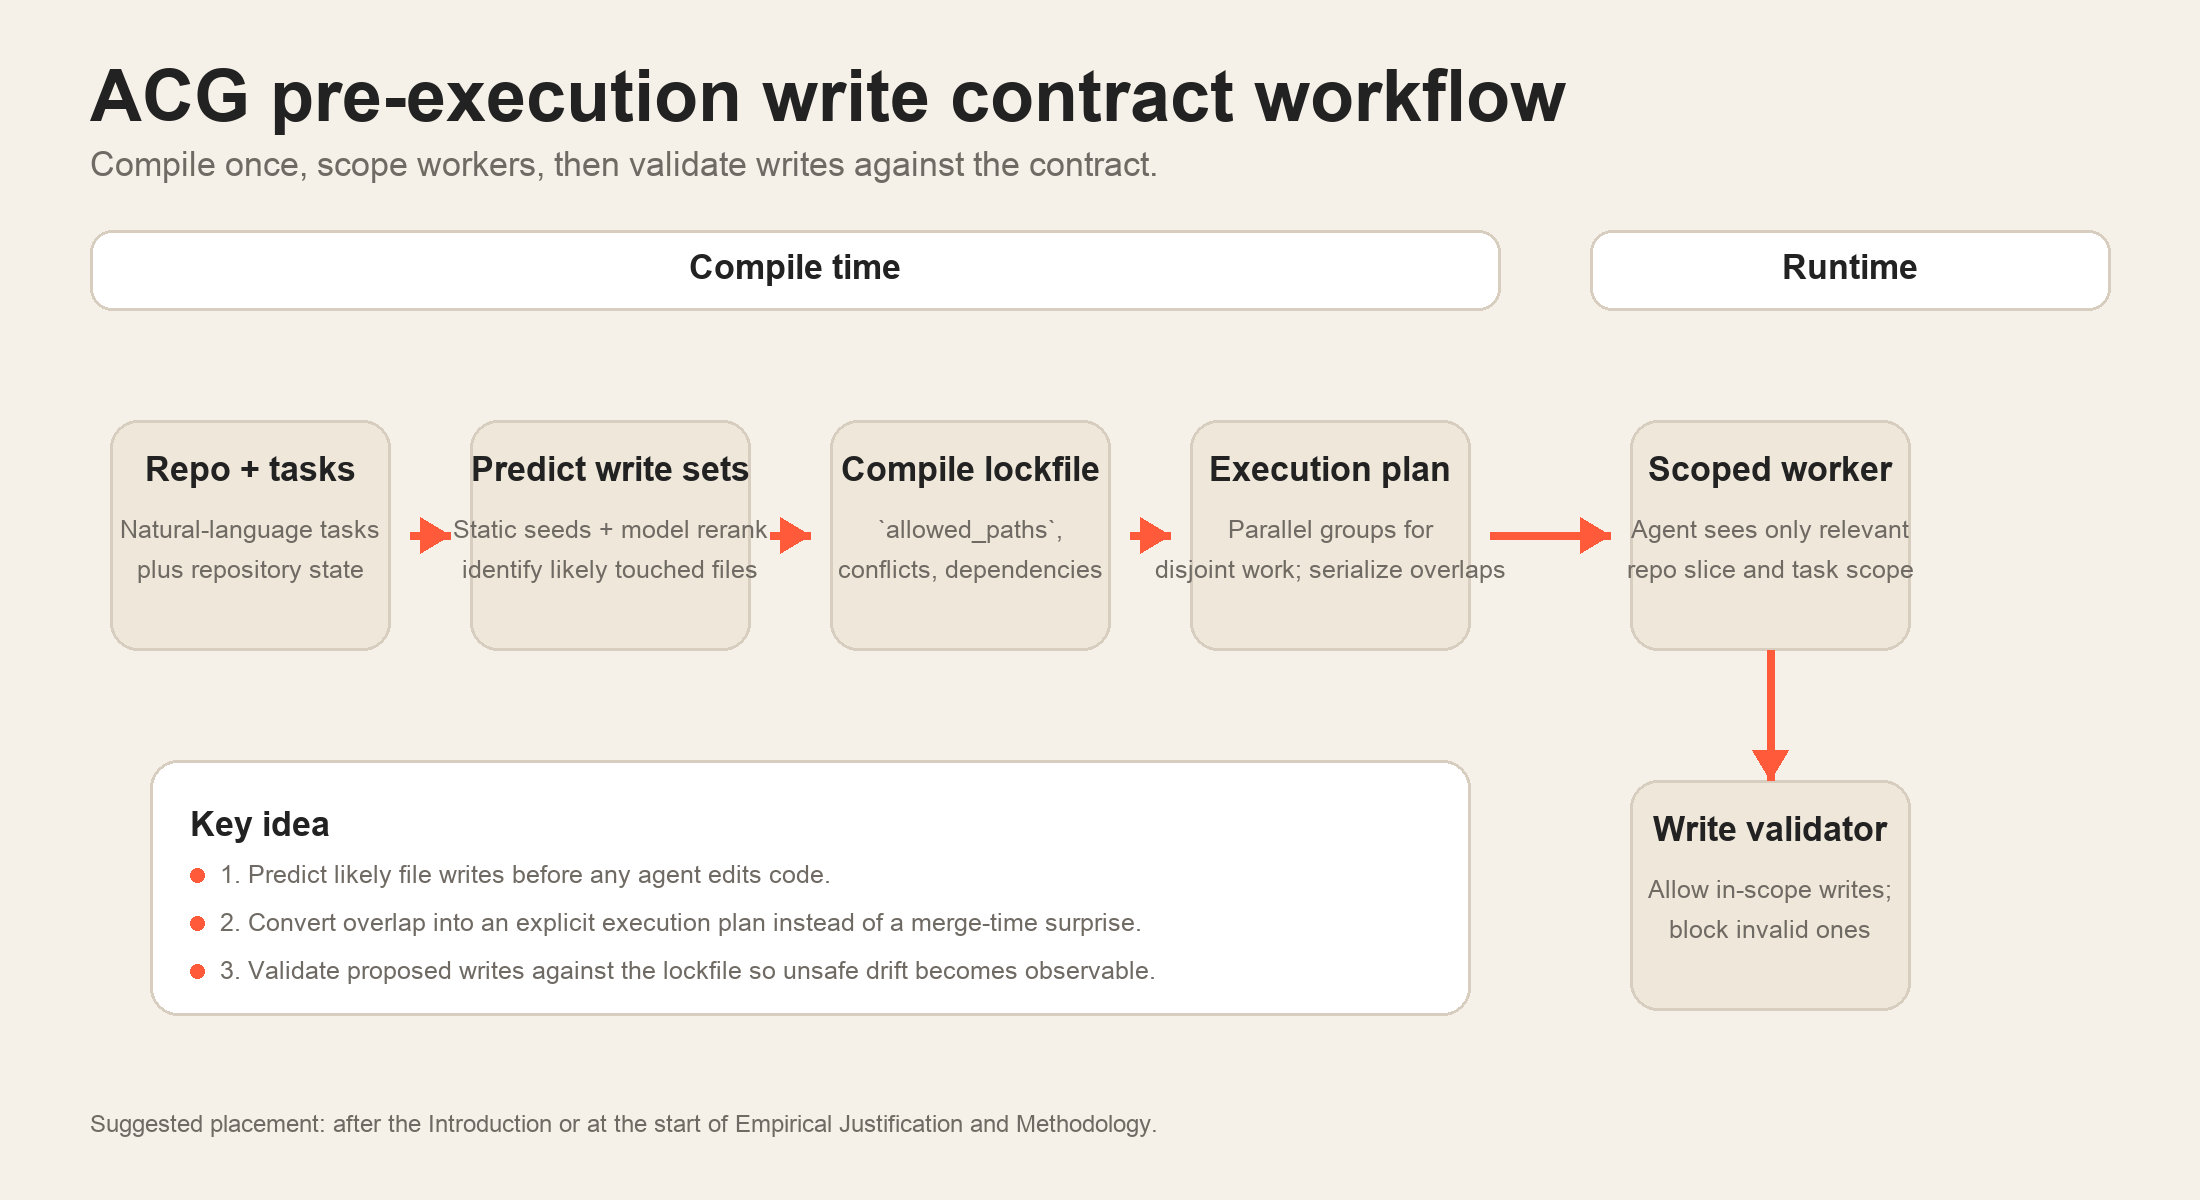
\includegraphics[width=\textwidth]{acg_workflow.png}
  \caption{Pre-execution write-contract workflow in ACG. Before any worker edits code, the system predicts likely write sets, compiles an \texttt{agent\_lock.json} contract, derives conflict-aware execution groups, and validates proposed writes against that contract at runtime.}
  \label{fig:acg-workflow}
\end{figure*}

% Figure 2: place in Token Efficiency.
\begin{figure*}[t]
  \centering
  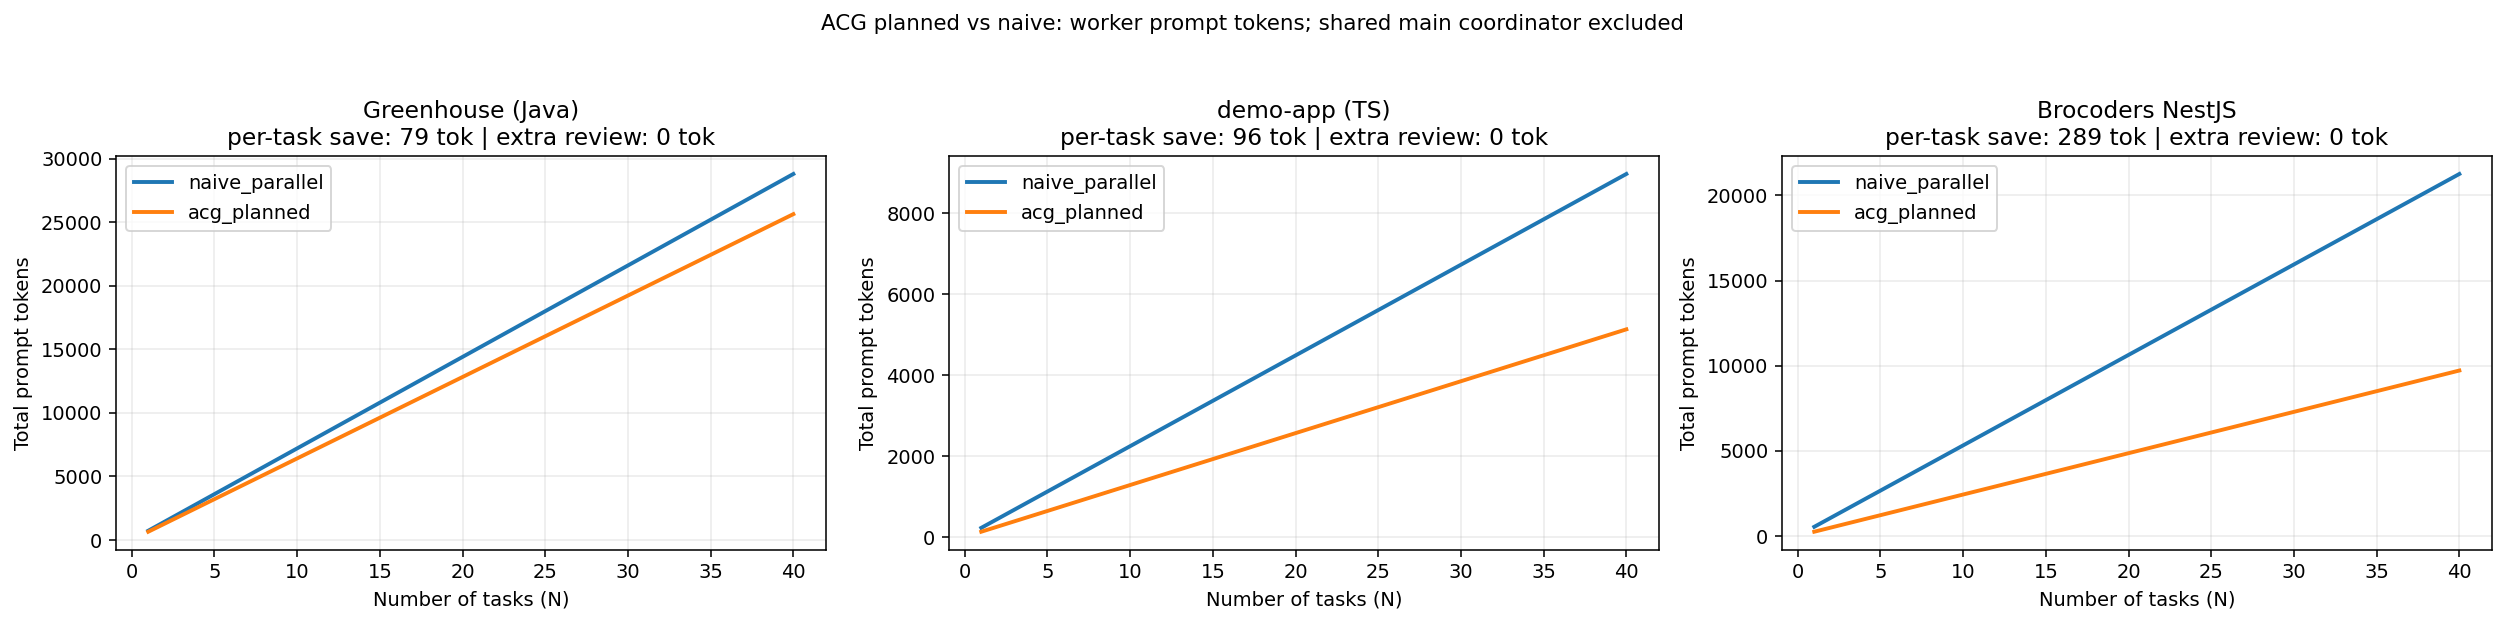
\includegraphics[width=\textwidth]{scaling_breakeven.png}
  \caption{Per-worker prompt-token savings from scoped execution across codebases. Savings vary by repository structure and lockfile tightness, but the direction is consistent: restricting worker context to the contracted scope reduces online prompt load.}
  \label{fig:token-savings}
\end{figure*}

% Figure 3: place in Validator Efficacy / Conflict Control.
\begin{figure*}[t]
  \centering
  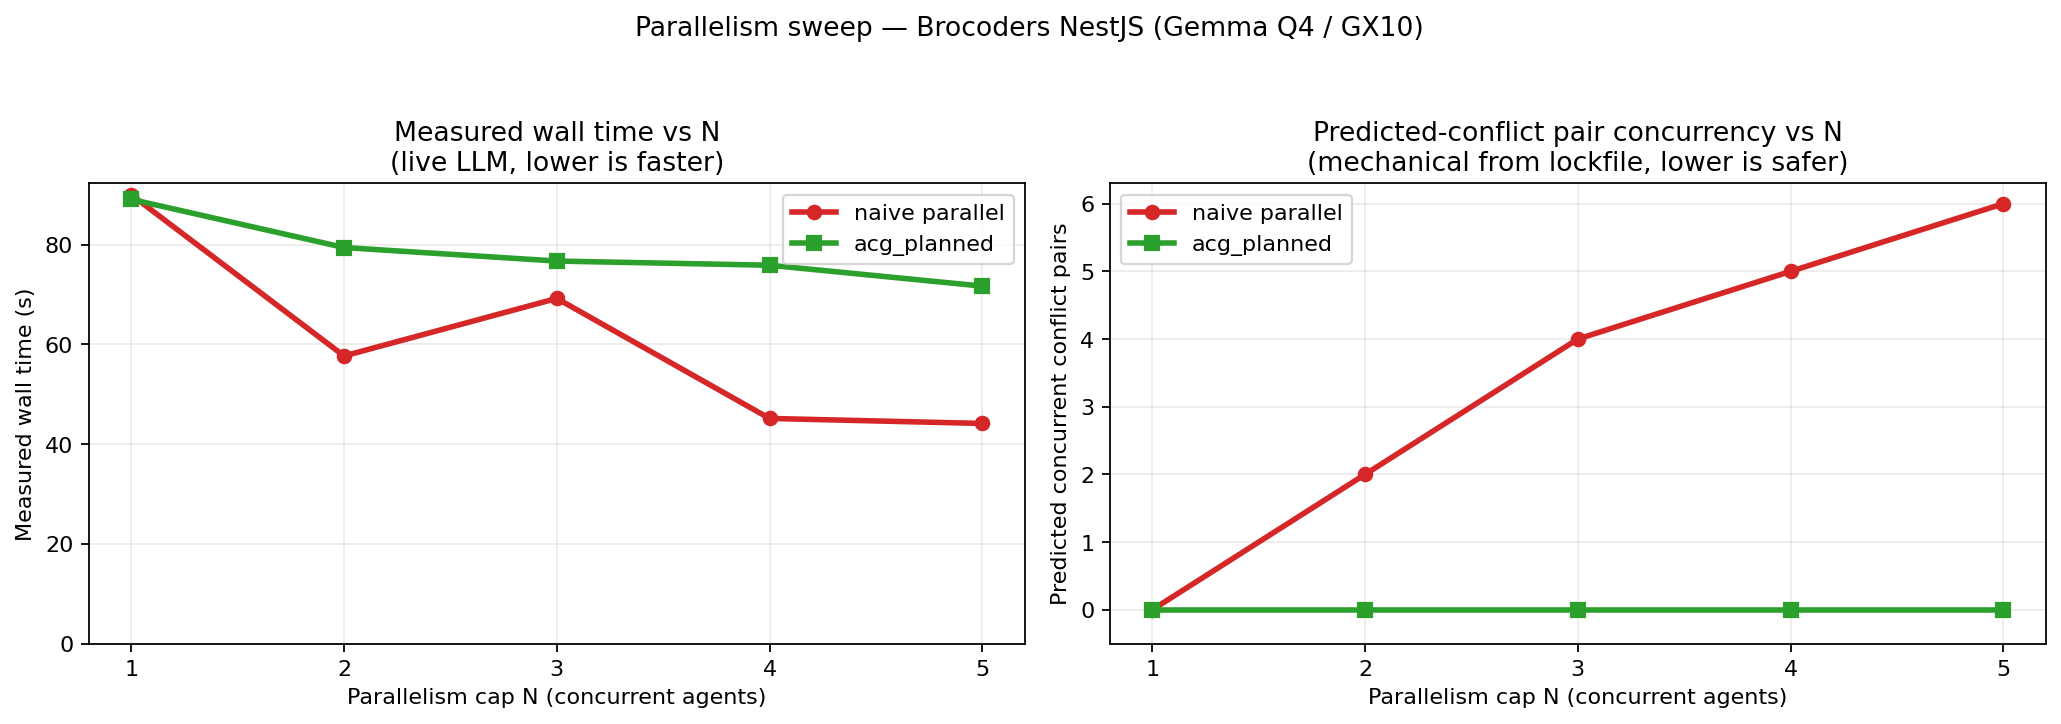
\includegraphics[width=\textwidth]{parallelism_sweep_brocoders.png}
  \caption{Parallelism trade-off on Brocoders NestJS. As naive concurrency increases, measured wall time falls but predicted concurrent-conflict pairs rise sharply. ACG preserves zero predicted concurrent conflicts by constraining execution to conflict-aware groups, even when that limits wall-time gains.}
  \label{fig:parallelism-sweep}
\end{figure*}

% Figure 4: place in Predictor vs. Agent.
\begin{figure*}[t]
  \centering
  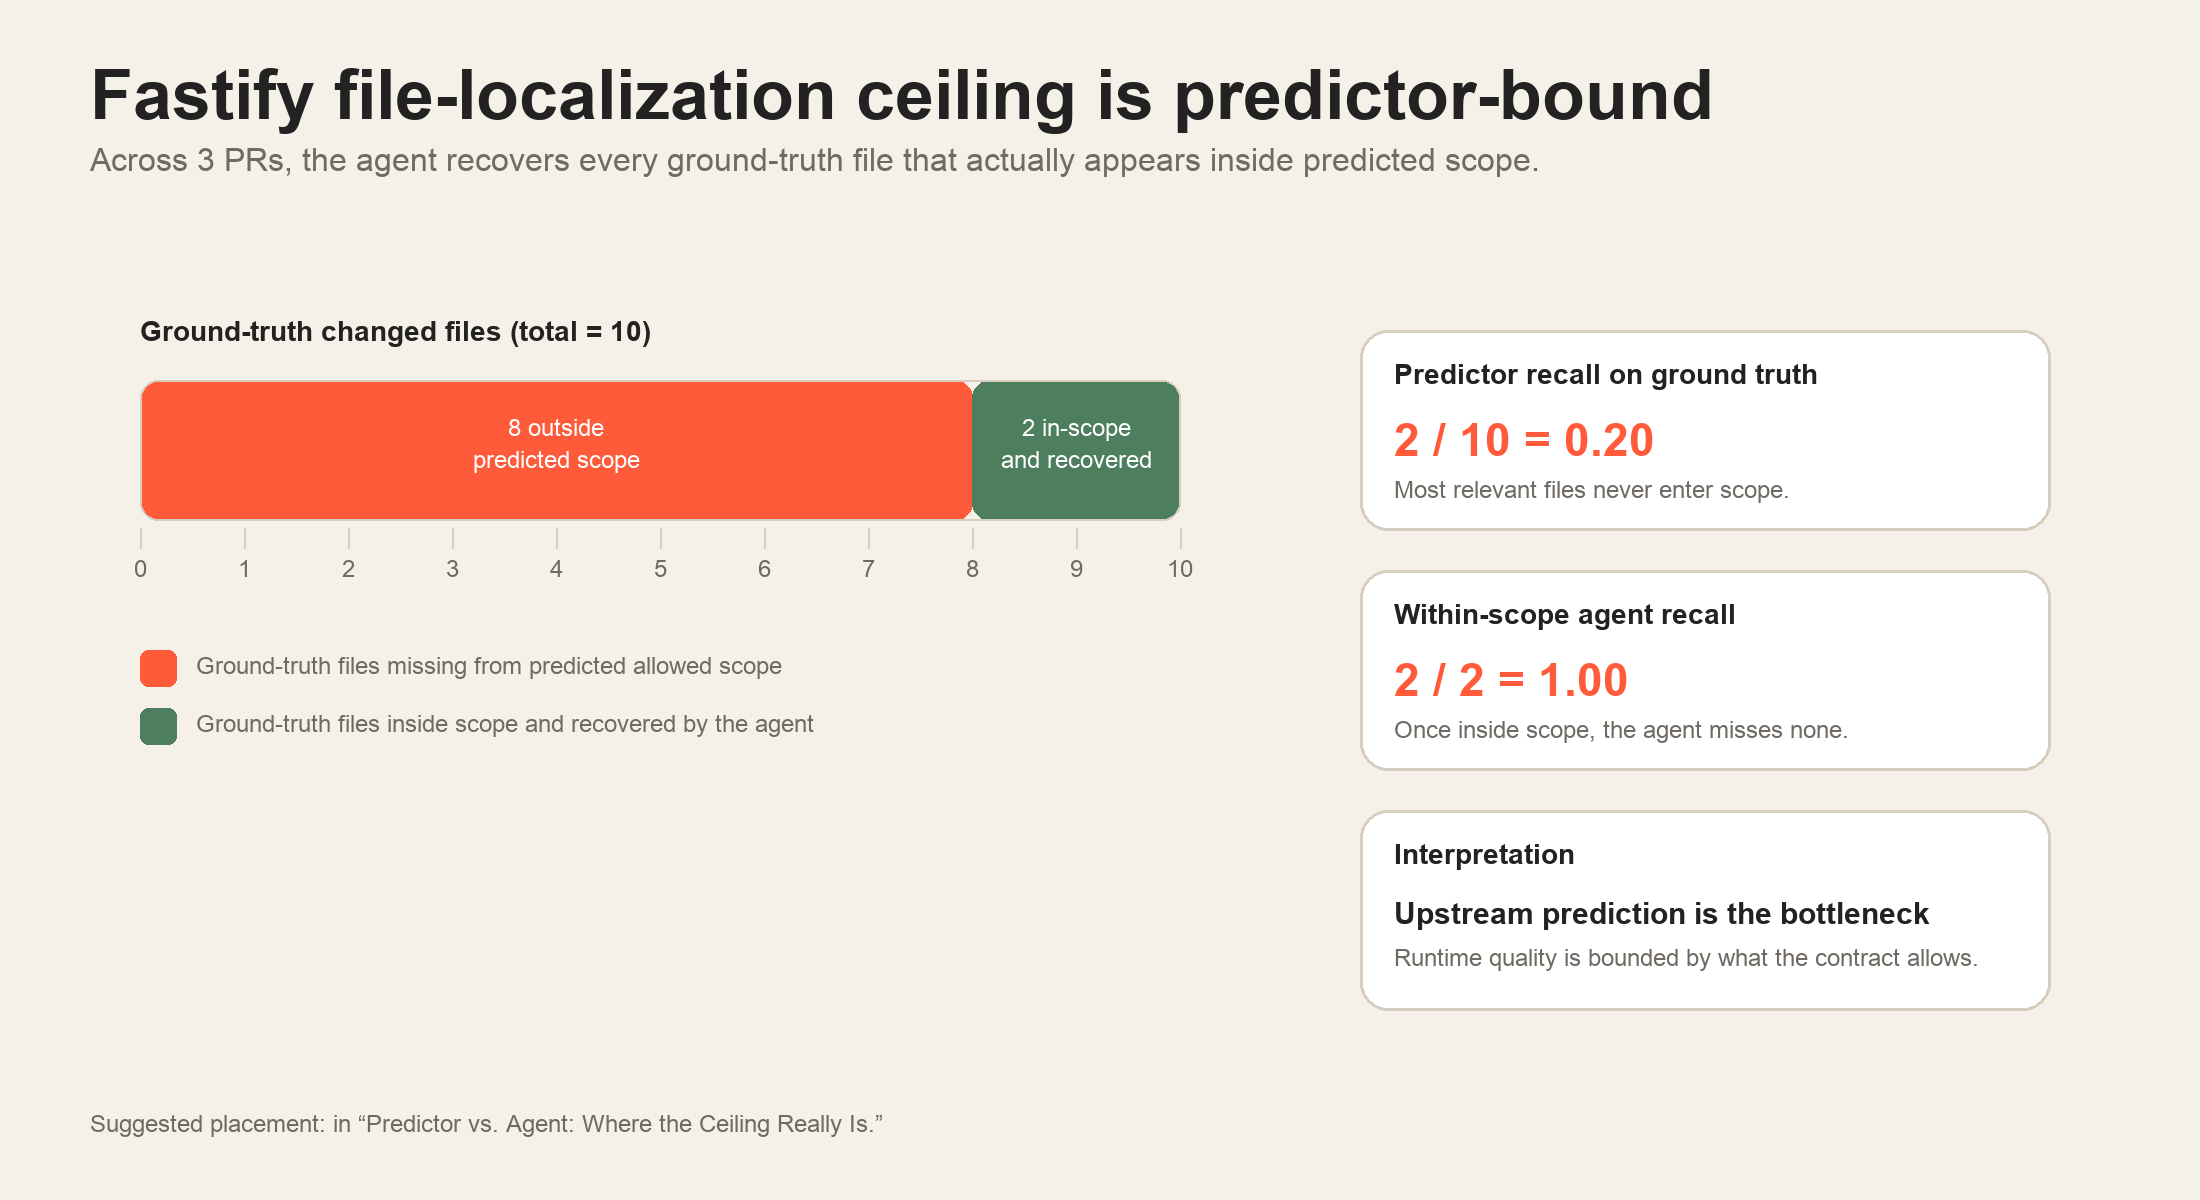
\includegraphics[width=\textwidth]{fastify_scope_decomposition.png}
  \caption{Fastify decomposition of the file-localization ceiling. Across three PRs, eight of ten ground-truth files fall outside predicted scope, while both in-scope ground-truth files are recovered by the agent. This supports the paper's claim that current performance is bounded primarily by predictor recall rather than by within-scope agent behavior.}
  \label{fig:fastify-decomposition}
\end{figure*}
